%\documentclass[handout]{beamer}
\documentclass[aspectratio=169]{beamer}
\usepackage{etex} % fixes new-dimension error

\input{macros/beamerconf}
\usepackage{etex} % fixes new-dimension error
\usepackage{lmodern} % fixes warnings
\usepackage{textcomp}% fixes warnings

\usepackage{graphicx,amsmath}
\usepackage{stmaryrd} % cf. interleave
%\usepackage{./macros/myisolatin1}
%\usepackage{./macros/prooftree}
\usepackage{alltt}
%\usepackage{./macros/circle}
\usepackage{listings}
\usepackage{relsize} % relative size fonts
\usepackage[normalem]{ulem} % strikethrough text (with \sout{.})
\usepackage{tikz}
\usetikzlibrary{%
  positioning
 ,patterns
 ,arrows
 ,automata
 ,calc
 ,shapes
 ,fit
 ,fadings
 ,decorations.pathreplacing
 ,plotmarks
% ,pgfplots.groupplots
 ,decorations.markings
}
% \tikzset{shorten >=1pt,node distance=2cm,on grid,auto,initial text={},inner sep=2pt}
\tikzstyle{aut}=[shorten >=1pt,node distance=2cm,on grid,auto,initial text={},inner sep=2pt]
\tikzstyle{st}=[circle,draw=black,fill=black!10,inner sep=3pt]
\tikzstyle{sst}=[rectangle,draw=none,fill=none,inner sep=3pt]
\tikzstyle{final}=[accepting]
\usepackage[normalem]{ulem} % striking out text with \sout{...}
\usepackage{xspace}

\usepackage{transparent}

% Nicer TT fonts
\usepackage[scaled=.83]{beramono}
\usepackage[T1]{fontenc}




%------ using eurosym -------------------------------------------------------
\usepackage{eurosym}
\def\inh#1{\mbox{\small\euro}_{#1}}
\def\eith#1#2{\mathopen{[}#1 \ ,#2\mathclose{]}}

%------ using xy ------------------------------------------------------------
\usepackage[all]{xy}
%\def\larrow#1#2#3{\xymatrix{ #3 & #1 \ar[l] _-{#2} }}
\def\larrow#1#2#3{\xymatrix{ #3 & #1 \ar[l] _--{#2} }}
\def\rarrow#1#2#3{\xymatrix{ #1 \ar[r]^-{#2} & #3 }}
\def\arLaw#1#2#3#4#5{
\xymatrix{
        #1      \ar@/^1pc/[rr]^-{#4} &
        #5 &
        #2      \ar@/^1pc/[ll]^-{#3}
}}
\def\arLeq#1#2#3#4{\arLaw{#1}{#2}{#3}{#4}\leq}
%------ using pstricks (rnode etc) ------------------------------------------
%\usepackage{pstricks,pst-node,pst-text,pst-3d}
\input{macros/macros}


\setLecture{5}{Behavioural equivalences}



\begin{document}

\frame[plain]{\titlepage}


% \section{Introduction}

\begin{slide}{Overview}

\begin{block}{Recall}
\begin{enumerate}
  \item Labelled Transition Systems:
    $\xymatrix{
      q_1 \ar[r]^{a}  & q_2 \ar@(ur,dr)[]^{b} 
    }$

  \item (Sequential) Process algebra:
    $P = a.Q ~~~~ Q=b.Q$

  \item Meaning of \structure{(2)} using \structure{(1)}

  \item Equivalence relations ((bi)simulations)
\end{enumerate}  
\end{block}

\begin{block}{Still missing}
\begin{itemize}
  \item \alert{\textbf{Interaction}} between processes
  \item \emph{Interaction \alert{diagrams}} vs. \emph{interacting \alert{processes}}
  \item Enrich \structure{(2)} and \structure{(3)}; expand \structure{(4)}
\end{itemize}
\end{block}

\end{slide}



\begin{slide}{Behavioural Equivalences -- Intuition}
\small


Two automata (or LTS) should be \alert{equivalent} if they cannot be distinguished by interacting with them.


\begin{block}{Equality of functional behaviour}
is not preserved by \structure{parallel} composition: non \structure{compositional} semantics, cf,
\begin{center}
\texttt{x:=4; x:=x+1} ~and~ \texttt{x:=5}
\end{center}
\end{block}

\begin{block}{Graph isomorphism} 
is too strong (why?)
\end{block}

\end{slide}



%----------------------------------------------------------------------------------
% \begin{slide}{Trace}
% \small

% \begin{block}{Definition}
% Let $T = \pair{S, \Act,  \rra}$ be a labelled transition system. The set of \alert{traces} $L_{s}$, for $s \in S$ is the minimal set  satisfying
% \begin{align*}
% \text{\structure{(1)}}\; \;  &  \epsilon \in L_{s}\\
% \text{\structure{(2)}}\; \;  &  a \cdot \sigma \in L_{s}\; \imp\; \rcb{\exists}{s'}{s' \in S}{s \rtran{a} s'\, \e\, \sigma \in L_{s'}}
% \end{align*}
% \end{block}


% \end{slide}

\section{EQ1 -- Language equivalence}

%----------------------------------------------------------------------------------
\begin{slide}{Language  equivalence}
\small

\begin{block}{Definition}
Two automata $A, B$ are \alert{language equivalent} iff  $ L_A =  L_B$\\
(i.e. if they can perform the same finite sequences of transitions)
\end{block}
~\\

\begin{example}
  \centering
  % Requires \usepackage{graphicx}
  \includegraphics[width=9cm]{./images/alarm3.pdf}
\end{example}


\alert{Language equivalence} applies  when one can neither interact with a system, nor distinguish a slow system from one that has come to a stand still.
\end{slide}


% \begin{slide}{Exercise}
%   \centering
%   \doExercise{Consider the system}{
%   \centering
%   \begin{tikzpicture}
%       \node(p){$p$}; \node[right=of p](p1){$p_1$}; \node[right=of p1](p2){$p_2$};
%       \draw[->] (p)edge[bend right] node[below]{a} (p1)
%                 (p1)edge[bend right] node[above]{b}(p)
%                 (p2)edge node[above]{d} (p1)edge[loop right] node[right]{c}(p1) ;
%   \end{tikzpicture}
%   \begin{enumerate}
%     \item Formalise the system as a tuple $(S,Act,\to)$
%     \item List 4 different traces from state (p2).
%   \end{enumerate}
%   }
% \end{slide}


\begin{slide}{Exercise}
  \centering
  \doExercise{Find pairs of automata with the same language}{
    \centering 
    \wrap{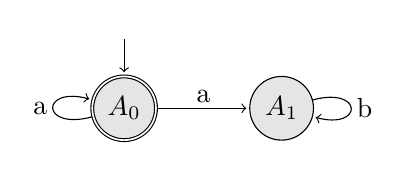
\begin{tikzpicture}[aut]
      \node[st,initial above,final]  (s_0) {$A_0$};
      \node[st] (s_1) [right of=s_0] {$A_1$};
      \path[->]
        (s_0) edge  node {a}  (s_1)
        (s_0) edge[loop left] node {a}  ()
        (s_1) edge[loop right] node {b}  (s_0);
    \end{tikzpicture}}
    ~~~~~~~~~~
    \wrap{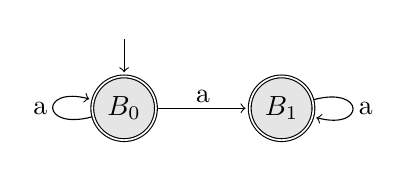
\begin{tikzpicture}[aut]
      \node[st,initial above,final]  (s_0) {$B_0$};
      \node[st,final] (s_1) [right of=s_0] {$B_1$};
      \path[->]
        (s_0) edge  node {a}  (s_1)
        (s_0) edge[loop left] node {a}  ()
        (s_1) edge[loop right] node {a}  (s_0);
    \end{tikzpicture}}
    ~~~~~~~~~
    \wrap{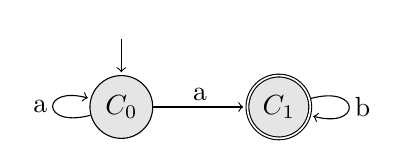
\begin{tikzpicture}[aut]
      \node[st,initial above]  (s_0) {$C_0$};
      \node[st,final] (s_1) [right of=s_0] {$C_1$};
      \path[->]
        (s_0) edge  node {a}  (s_1)
        (s_0) edge[loop left] node {a}  ()
        (s_1) edge[loop right] node {b}  (s_0);
    \end{tikzpicture}}
    ~~~~~~~~~
    \wrap{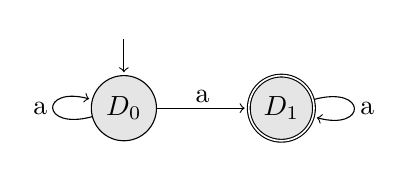
\begin{tikzpicture}[aut]
      \node[st,initial above]  (s_0) {$D_0$};
      \node[st,final] (s_1) [right of=s_0] {$D_1$};
      \path[->]
        (s_0) edge  node {a}  (s_1)
        (s_0) edge[loop left] node {a}  ()
        (s_1) edge[loop right] node {a}  (s_0);
    \end{tikzpicture}}
    ~~~~~~~~~
    \wrap{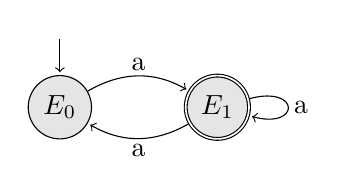
\begin{tikzpicture}[aut]
      \node[st,initial above]  (s_0) {$E_0$};
      \node[st,final] (s_1) [right of=s_0] {$E_1$};
      \path[->]
        (s_0) edge[bend left]  node {a}  (s_1)
        (s_1) edge[bend left]  node {a}  (s_0)
        (s_1) edge[loop right] node {a}  (s_0);
    \end{tikzpicture}}

  }
\end{slide}


\section{EQ2 -- Similarity}

%----------------------------------------------------------------------------------
\begin{slide}{Simulation}
\begin{flushright}
the quest for a \alert{behavioural equality}:\\
able to identify states that cannot be distinguished by any \alert{realistic} form of  observation
\end{flushright}
~\\

\small
\begin{block}{Simulation}
\caixa{A state $q$ \alert{simulates} another state $p$
\alert{if}\\
every transition from $q$ is corresponded by a transition from $p$
\alert{and}\\
this capacity is kept along the whole life of the system to which state space $q$ belongs to.}
\end{block}
\end{slide}

%----------------------------------------------------------------------------------
\begin{slide}{Simulation}
\small

\begin{block}{Definition}
Given  $\pair{S_1, \Act, \rra_1}$  and $\pair{S_2, \Act, \rra_2}$
 over $\Act$ \faded{(ignoring initial and final states)}
a relation \structure{$R \subseteq S_1 \times S_2$} is a \structure{simulation} iff,
for all $\pair{p,q} \in \structure{R}$ and $a \in \Act$,

\begin{align*}
%\text{\gold{(1)}}\; \;  & p \downarrow_1 \;  \imp\; q \downarrow_2\\ &\\
\text{\gold{(1)}}\; \;  & p \rtran{a}_1 p'\;  \imp\; \rcb{\exists}{q'}{q' \in S_2}{q \rtran{a}_2 q'\, \e\, \pair{p',q'} \in \structure{R}}   
\end{align*}
\vspace{0mm}

\begin{equation*}
\xymatrix{
p \ar[d]^-{a} & \hspace{-1.5cm} \structure{R}  & \hspace{-2.7cm} q 
  & \!\! \text{\raisebox{-10mm}{\Huge $\imp$}} \! \! &  &  &  q \ar[d]^-{a} \\
p'           &   &           &                                   & p'\hspace{-2.7cm} &  \structure{R} \hspace{-1.5cm} &  q'
}
\end{equation*}

\end{block}
\end{slide}

%----------------------------------------------------------------------------------
\begin{slide}{Example}

\begin{exampleblock}{\exercise Find simulations}
\begin{equation*}
\xymatrix{
& q_1  \ar[r]^{d} & q_2 &       &        &                              p_2\\
q_0 \ar[ru]^{a} \ar[rd]_{a} &  & & p_0 \ar[r]^{a} & p_1 \ar[ru]^{d} \ar[rd]_{e} & \\
& q_4  \ar[r]_{e} & q_3 &       &        &                              p_3\\
}
\end{equation*}
\end{exampleblock}

\vspace{0.2cm}
\visible<2->{\exerciseBack\begin{equation*}
q_0 \lesssim p_0 \text{\hspace{0.5cm} cf. \hspace{0.3cm}} 
\enset{\pair{q_0,p_0}, \pair{q_1,p_1},\pair{q_4,p_1},\alert{\ldots}} %\pair{q_2,p_2},\pair{q_3,p_3}}
\end{equation*}}
\end{slide}

\exerciseAdd


%----------------------------------------------------------------------------------
\begin{slide}{Similarity}
\small

\begin{block}{Definition}
\centering
\[p \lesssim q\; \equiv\; \rcb{\exists}{R}{}{R\; \text{is a simulation and}\; \pair{p,q} \in R} 
\]
\emph{We say \alert{$p$ is simulated by $q$}.}
\end{block}

% \begin{block}{Automata simulation}
%   \[\pair{S_1,\set{s_1},\dda_1,\rra_1} \lesssim \pair{S_2,\set{s_2},\dda_2,\rra_2}\; \equiv\; s_1 \lesssim s_2 
% \]
% \end{block}

\begin{block}{Lemma}
The similarity relation is a preorder\\
\faded{(ie, reflexive and transitive)}
\end{block}
\end{slide}


\section{EQ3 -- Bisimilarity}
%----------------------------------------------------------------------------------
\begin{slide}{Bisimulation}
\small

\begin{block}{Definition}
Given  $\pair{S_1, \Act,  \rra_1}$  and $\pair{S_2, \Act, \rra_2}$ over $\Act$,
relation $R \subseteq S_1 \times S_2$ is a \structure{bisimulation} iff both $R$ and its converse $\aconv{R}$
are simulations.

I.e.,
whenever $\pair{p,q} \in R$ and $a \in \Act$,

\begin{align*}
%\text{\gold{(1)}}\; \;  &  p \downarrow_1 \;  \dimp\; q \downarrow_2\\ &\\
\text{\gold{(1)}}\; \;  & p \rtran{a}_1 p'\; \imp\; \rcb{\exists}{q'}{q' \in S_2}{q \rtran{a}_2 q'\, \e\, \pair{p',q'} \in R}   \\
\text{\gold{(2)}}\; \;  & q \rtran{a}_2 q'\; \imp\; \rcb{\exists}{p'}{p' \in S_1}{p \rtran{a}_1 p'\, \e\, \pair{p',q'} \in R}   
\end{align*}

%\begin{equation*}
%\xymatrix{
%p \ar[d]^-{a} & \hspace{-1.5cm} R  & \hspace{-2.7cm} q
%    & \! \! \text{\raisebox{-10mm}{\Huge $\Leftrightarrow$}} \! \! &   &  
%    &  q \ar[d]^-{a} \\
%p'           &   &           &                                   & p'\hspace{-2.7cm} &  R \hspace{-1.5cm} &  q'
%}
%\end{equation*}
\centering
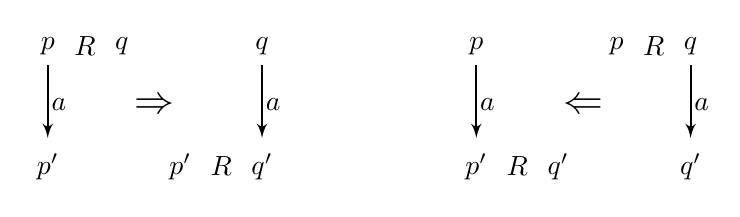
\begin{tikzpicture}[%
    every edge/.style={draw, thick,-latex',shorten >= 2pt}]
  \tikzstyle{l} = [auto,inner sep=1pt]
  % the square
  \node(p){$p$};\node[right=2.3 of p](q2){$q$};
  \node[below=1 of p](p'){$p'$};\node(q')at(p'-|q2){$q'$};
  % the R parts
  \node[right=0 of p](R1){$R$};\node[right=0 of R1](q){$q$};
  \node[left=0 of q'](R2){$R$};\node[left=0 of R2](p'2){$p'$};
  % the arrows
  \draw[->] (p)edge node[l]{$a$}(p') (q2)edge node[l]{$a$}(q');
  \node at ($(p)!.5!(q')$){{\Large $\Rightarrow$}};
  %%%%%%%
  % the square
  \node[right=2.3 of q2](pp){$p$};\node[right=2.3 of pp](q2){$q$};
  \node[below=1 of pp](p'){$p'$};\node(q')at(p'-|q2){$q'$};
  % the R parts
  \node[right=0 of p'](R1){$R$};\node[right=0 of R1](q){$q'$};
  \node[left=0 of q2](R2){$R$};\node[left=0 of R2](p'2){$p$};
  % the arrows
  \draw[->] (pp)edge node[l]{$a$}(p') (q2)edge node[l]{$a$}(q');
  \node at ($(pp)!.5!(q')$){{\Large $\Leftarrow$}};

\end{tikzpicture}

\end{block}
\end{slide}



%----------------------------------------------------------------------------------
\begin{slide}{Examples}

\begin{exampleblock}{\exercise Find bisimulations that include $q_1$}
\begin{equation*}
\xymatrix{
& q_1  \ar[ld]_{a}  \ar[rd]^{a} & & & & m \ar[d]_{a}\\
q_2 \ar[rr]^{c}  && q_3 \ar@(ur,dr)[]^{c}  & & & n\ar@(ur,dr)[]^{c}
}
\end{equation*}
% R = \enset{(q_1,m), (q_2, n), (q_3,n) }
\vspace{1cm}

\begin{equation*}
\xymatrix{
q_1 \ar[r]^{a} & q_2  \ar[r]^{a}  & q_3  \ar[r]^{a} & \cdots & & h\ar@(ur,dr)[]^{a}  \\
}
\end{equation*}
% R = \setdef{q_i, h}{i \geq 1}  
\end{exampleblock}

\end{slide}


%----------------------------------------------------------------------------------
\begin{slide}{Examples}

\begin{exampleblock}{\exercise Find bisimulations that include $q_1$}
\vspace*{-3mm}
\begin{equation*}
\xymatrix{
& q_1  \ar[ld]_{a}  \ar[rd]^{a} & & & & p_1  \ar[d]^{a} \\
q_2 \ar[d]^{c}  && q_3  \ar[d]^{c}  & && p_2  \ar[ld]_{c}  \ar[rd]^{c} & \\
q_4 & & q_5 & &p_4 & & p_5\\
& q_1  \ar[ld]_{a}  \ar[rd]^{a} & & & & p_1  \ar[d]^{a} \\
q_2 \ar[d]^{\rdb{b}}  && q_3  \ar[d]^{c}  & && p_2  \ar[ld]_{\rdb{b}}  \ar[rd]^{c} & \\
q_4 & & q_5 & &p_4 & & p_5
}
\end{equation*}
\end{exampleblock}
\end{slide}


% Definition
% p∼q ≡ ⟨∃R :: Risabisimulationand⟨p,q⟩∈R⟩
%----------------------------------------------------------------------------------
\begin{slide}{Bisimilarity}
\small

\begin{block}{Definition}
\centering
\[p \sim q\; \equiv\; \rcb{\exists}{R}{}{R\; \text{is a bisimulation and}\; \pair{p,q} \in R} 
\]
\emph{We say \alert{$p$ is bisimilar to $q$}.}
\end{block}


\begin{block}{Lemma}
\centering
Two processes $P$ and $Q$ are bisimilar if there is a bisimulation that includes $\pair{P,Q}$.
\end{block}

% \begin{block}{Automata simulation}
%   \[\pair{S_1,\set{s_1},\dda_1,\rra_1} \lesssim \pair{S_2,\set{s_2},\dda_2,\rra_2}\; \equiv\; s_1 \lesssim s_2 
% \]
% \end{block}

% \begin{block}{Lemma}
% The similarity relation is a preorder\\
% \faded{(ie, reflexive and transitive)}
% \end{block}
\end{slide}
%----------------------------------------------------------------------------------
% \begin{slide}{After thoughts}
% \small


% \begin{itemize}
% \item Follows a \gold{$\forall, \exists$ pattern}: $p$ in all its transitions challenge $q$ which is called to find a match to each of those (and conversely)
% \item Tighter correspondence with transitions
% \item Based on the information that the transitions convey, rather than on the shape of the LTS
% \item \gold{Local} checks on states
% \item \gold{Lack of hierarchy}  on the pairs of the bisimulation (no temporal order on the checks is required)
% \end{itemize}
% which means \gold{bisimilarity can be used to reason about infinite or circular behaviours}.
% \end{slide}

% %----------------------------------------------------------------------------------
% \begin{slide}{After thoughts}
% \small
% ~\\

% \noindent
% Compare the definition of bisimilarity with 
% ~\\
% ~\\


% $p == q$ if, for all $a  \in \Act$
% \begin{align*}
% %\text{\gold{(1)}}\; \;  &  p \downarrow_1 \;  \dimp\; q \downarrow_2\\ &\\
% \text{\gold{(1)}}\; \;  & p \rtran{a}_1 p'\; \imp\; \rcb{\exists}{q'}{q' \in S_2}{q \rtran{a}_2 q'\, \e\, p' == q'}   \\
% \text{\gold{(2)}}\; \;  & q \rtran{a}_2 q'\; \imp\; \rcb{\exists}{p'}{p' \in S_1}{p \rtran{a}_1 p'\, \e\, p' == q'}    
% \end{align*}

% \end{slide}

% %----------------------------------------------------------------------------------
% \begin{slide}{After thoughts}
% \small
% ~\\


% $p == q$ if, for all $a  \in \Act$
% \begin{align*}
% %\text{\gold{(1)}}\; \;  &  p \downarrow_1 \;  \dimp\; q \downarrow_2\\ &\\
% \text{\gold{(1)}}\; \;  & p \rtran{a}_1 p'\; \imp\; \rcb{\exists}{q'}{q' \in S_2}{q \rtran{a}_2 q'\, \e\, p' == q'}   \\
% \text{\gold{(2)}}\; \;  & q \rtran{a}_2 q'\; \imp\; \rcb{\exists}{p'}{p' \in S_1}{p \rtran{a}_1 p'\, \e\, p' == q'}    
% \end{align*}

% \gry{
% \begin{itemize}
% \item The meaning of $==$ on the pair $\pair{p,q}$ requires having already established the meaning of $==$ on the derivatives
% \item ... therefore the definition is \gold{ill-founded} if the state space reachable from $\pair{p,q}$ is infinite or contain loops
% \item ... this is a \gold{local} but \gold{inherently inductive} definition (to revisit later)
% \end{itemize}
% }
% \end{slide}



% %----------------------------------------------------------------------------------
% \begin{slide}{After thoughts}
% \small

% \begin{block}{Proof method}

% To prove that two behaviours are bisimilar, find a bisimulation containing them ...



% \begin{itemize}
% \item
% ... \gold{impredicative} character
% \item \gold{coinductive} vs \gold{inductive} definition
% \end{itemize}
% \end{block}
% \end{slide}

% %----------------------------------------------------------------------------------
% \begin{slide}{Properties}
% \small

% \begin{block}{Definition}
% \[p \sim q\; \equiv\; \rcb{\exists}{R}{}{R\; \text{is a bisimulation and}\; \pair{p,q} \in R} 
% \]
% \end{block}
% \begin{block}{Lemma}
% \begin{enumerate}
% \item The identity relation $\id$ is a bisimulation
% \item The empty relation $\bot$ is a bisimulation
% \item The converse $\aconv{R}$ of a bisimulation is a bisimulation
% \item The composition $S \comp R$ of two bisimulations $S$ and $R$ is a bisimulation
% \item The $\bigcup_{i \in I} R_i$ of a family of bisimulations
%  $\setdef{R_i}{i \in I}$ is a bisimulation
% \end{enumerate}
% \end{block}
% \end{slide}

% %----------------------------------------------------------------------------------
% \begin{slide}{Properties}

% \small


% \begin{block}{Lemma}
% The bisimilarity relation is an equivalence relation\\
% \gry{(ie, reflexive, symmetric and transitive)}
% \end{block}

% \begin{block}{Lemma}
% The class of all bisimulations between two LTS has the structure of a 
% \structure{complete lattice}, ordered by set inclusion, whose top is the  \structure{bisimilarity} relation $\sim$.
% \end{block}
% \end{slide}

% %----------------------------------------------------------------------------------
% \begin{slide}{Properties}

% \small


% \begin{block}{Lemma}
% In a \gold{deterministic} labelled transition system, two states are bisimilar iff they are trace equivalent, i.e.,
% $$
% s \obs s'\; \; \dimp\;\; L_{s} = L_{s'}
% $$
% ~\\

% \gry{Hint: define a relation $R$ as 
% $$\pair{x,y} \in R \; \dimp\;  L_{x} = L_{y}$$
%  and show $R$ is a bisimulation.}
% \end{block}


% \end{slide}

%----------------------------------------------------------------------------------
\begin{slide}{Properties}
\centering
\begin{alertblock}{Warning}
\centering
% \fbox{The bisimilarity relation \structure{$\sim$} \rdb{is not} the \structure{symmetric closure of $\lesssim$}}
\fbox{$\Big[p\lesssim q$ and $q\lesssim p\Big]$ does \rdb{not} imply
  $\Big[p \sim q\Big]$}
\end{alertblock}

% ~\\[5mm]
% i.e., $\Big[p\lesssim q$ and $q\lesssim p\Big]$ does \rdb{not} imply
%   $\Big[p \sim q\Big]$
\end{slide}


%----------------------------------------------------------------------------------
\begin{slide}{Properties}

\small

\begin{alertblock}{Warning}
\centering
$\Big[p\lesssim q$ and $q\lesssim p\Big]$ does \rdb{not} imply
  $\Big[p \sim q\Big]$
% \fbox{The bisimilarity relation \structure{$\sim$} \rdb{is not} the \structure{symmetric closure of $\lesssim$}}
\end{alertblock}

\begin{example}
\begin{center}
$q_0 \lesssim p_0,\;  p_0 \lesssim q_0\;\;\; \text{but}\;\;\;  p_0 \not \sim q_0$
\end{center}

\begin{equation*}
\xymatrix{
& q_1  & & & & \\
q_0 \ar[ru]^{a} \ar[rd]^{a} &  & & p_0 \ar[r]^{a} & p_1 \ar[r]^{b} & p_3\\
& q_2  \ar[r]^{b} & q_3 &       &        &                          
}
\end{equation*}
\end{example}
\end{slide}




%----------------------------------------------------------------------------------
\begin{slide}{Notes}
\small
\begin{block}{Similarity as the \underline{greatest} simulation}
\begin{equation*}
\structure{\lesssim}\;  \deff\; \bigcup \setdef{S}{S\, \text{is a simulation}} 
\end{equation*}
\end{block}
\begin{block}{Bisimilarity as the \underline{greatest} bisimulation}
\begin{equation*}
\structure{\sim}\;  \deff\; \bigcup \setdef{S}{S\, \text{is a bisimulation}} 
\end{equation*}
\end{block}
%\begin{flushright}
%cf \gold{relational} translation of definitions\\
%$\structure{\lesssim}$ and $\structure{\sim}$ as \gold{greatest fix points} (Tarski's theorem)
%\end{flushright}
\end{slide}

%-------------------------------------------------------------------------------

\begin{slide}{Exercises}
\frsplit{
\begin{exampleblock}{\exercise P,Q Bisimilar?}
 \vspace*{-4mm}
 \begin{align*}
  \mathbf{P}&=a.P_1\\
  P_1&=b.P + c.P\\[3mm]
  \mathbf{Q}&=a.Q_1\\
  Q_1&=b.Q_2+c.Q\\
  Q_2&=a.Q_3\\
  Q_3&=b.Q+c.Q_2
 \end{align*} 
\end{exampleblock}
}{
\begin{exampleblock}{\exercise P,Q Bisimilar?}
 \vspace*{-4mm}
 \begin{align*}
  \mathbf{P}&=a.(b.\cnil+\cnil)\\[3mm]
  \mathbf{Q}&=a.b.\cnil
 \end{align*}  
\end{exampleblock}

\begin{exampleblock}{\exercise P,Q Bisimilar?}
 \vspace*{-4mm}
 \begin{align*}
  \mathbf{P}&=a.(b.\cnil+c.\cnil)\\[3mm]
  \mathbf{Q}&=a.b.\cnil + a.c.\cnil
 \end{align*}  
\end{exampleblock}
}
Draw their LTS. If bisimilar, find the bisimulation.
\end{slide}

%-------------------------------------------------------------------------------

\begin{slide}{Exercises}
\begin{exampleblock}{\exercise Find a bisimulation}
%\vspace*{-3mm}
\frsplit{\centering
  \includegraphics{images/LTS-1}
}{\centering
  \includegraphics{images/LTS-2}
}
\end{exampleblock}
\end{slide}
%Rania Khalaf (IBM T.J. Watson Research Center, USA) - rkhalaf@us.ibm.com 

%-------------------------------------------------------------------------------
% \begin{slide}{More bisimulations}
% \small

% \myblock{Considering $\tau$-transitions}

% \begin{block}{Weak transition}
% \begin{align*}
%   p \Trans{\alpha} q ~~~&\text{iff}~~~
%   p \,(\rtran{\tau})^{*}\, q_1\rtran{a} q_2 \,(\rtran{\tau})^{*}\, q
%   \\
%   p \Trans{\tau} q ~~~&\text{iff}~~~
%   p \,(\rtran{\tau})^{*}\, q
% \end{align*}  
% where $\alpha \neq \tau$ and $(\rtran{\tau})^{*}$ is the reflexive and transitive closure of $\rtran{\tau}$.
% \end{block}

% \begin{block}{Weak bisimulation (vs. strong)}
% Given  $\pair{S_1, \Act,  \rra_1}$  and $\pair{S_2, \Act, \rra_2}$ over $\Act$,
% relation $R \subseteq S_1 \times S_2$ is a \structure{bisimulation} iff for all $\pair{p,q} \in R$ and $a \in \Act\,\rdb{\cup \set{\tau}}$,
% %
% \begin{align*}
% %\text{\gold{(1)}}\; \;  &  p \downarrow_1 \;  \dimp\; q \downarrow_2\\ &\\
% \text{\gold{(1)}}\; \;  & p \rtran{a}_1 p'\; \imp\;
%   \rcb{\exists}{q'}{q' \in S_2}{\rdb{q \Trans{a}_2  q'}\, \e\,
%   \pair{p',q'} \in R}   \\
% \text{\gold{(2)}}\; \;  & q \rtran{a}_2 q'\; \imp\;
%   \rcb{\exists}{p'}{p' \in S_1}{\rdb{p \Trans{a}_1 p'}\, \e\,
%   \pair{p',q'} \in R}   
% \end{align*}
% %\centering
% %\begin{tikzpicture}[%
% %    every edge/.style={draw, thick,-latex',shorten >= 2pt}]
% %  \tikzstyle{l} = [auto,inner sep=1pt]
% %  % the square
% %  \node(p){$p$};\node[right=2.3 of p](q2){$q$};
% %  \node[below=1 of p](p'){$p'$};\node(q')at(p'-|q2){$q'$};
% %  % the R parts
% %  \node[right=0 of p](R1){$R$};\node[right=0 of R1](q){$q$};
% %  \node[left=0 of q'](R2){$R$};\node[left=0 of R2](p'2){$p'$};
% %  % the arrows
% %  \draw[->] (p)edge node[l]{$a$}(p') (q2)edge node[l]{$a$}(q');
% %  \node at ($(p)!.5!(q')$){{\Large $\Rightarrow$}};
% %  %%%%%%%
% %  % the square
% %  \node[right=2.3 of q2](pp){$p$};\node[right=2.3 of pp](q2){$q$};
% %  \node[below=1 of pp](p'){$p'$};\node(q')at(p'-|q2){$q'$};
% %  % the R parts
% %  \node[right=0 of p'](R1){$R$};\node[right=0 of R1](q){$q'$};
% %  \node[left=0 of q2](R2){$R$};\node[left=0 of R2](p'2){$p$};
% %  % the arrows
% %  \draw[->] (pp)edge node[l]{$a$}(p') (q2)edge node[l]{$a$}(q');
% %  \node at ($(pp)!.5!(q')$){{\Large $\Leftarrow$}};
% %\end{tikzpicture}
% \end{block}
% \end{slide}



% \begin{slide}{More bisimulations}
% \small
% \myblock{Considering $\tau$-transitions}


% \begin{block}{Branching bisimulation}
% Given  $\pair{S_1, \Act,  \rra_1}$  and $\pair{S_2, \Act, \rra_2}$ over $\Act$,
% relation $R \subseteq S_1 \times S_2$ is a \structure{bisimulation} iff for all $\pair{p,q} \in R$ and $a \in \Act\,\rdb{\cup\set{\tau}}$,
% %
% \begin{align*}
% %\text{\gold{(1)}}\; \;  &  p \downarrow_1 \;  \dimp\; q \downarrow_2\\ &\\
% &\text{\gold{(1)} if}\; \;   p \rtran{a}_1 p'\; \text{then either}
%   \\&~~
%   \text{\gold{(1.1)}~} a=\tau \text{~and~}\pair{p',q}\in R \text{~~or}
%   \\&~~
%   \text{\gold{(1.2)}~}
%     \rcb{\exists}{q',q'' \in S_2}{}{\rdb{q \,(\trans{\tau}_2)^{*}\,q' \tran{a}_2  q''}\, \e\,
%     \pair{p,q'} \in R \e\,
%     \pair{p',q''} \in R} \\[3mm]
% %&\text{\gold{(2)} if}\; \;   q \rtran{a}_2 q'\; \imp\;
% %  \rcb{\exists}{p'}{p' \in S_1}{\rdb{p \Trans{a}_1 p'}\, \e\,
% %  \pair{p',q'} \in R}   
% &\text{\gold{(2)} if}\; \;   q \rtran{a}_2 q'\; \text{then either}
%   \\&~~
%   \text{\gold{(2.1)}~} a=\tau \text{~and~}\pair{p',q'}\in R \text{~~or}
%   \\&~~
%   \text{\gold{(2.2)}~}
%     \rcb{\exists}{p',p'' \in S_1}{}{\rdb{p \,(\trans{\tau}_1)^{*}\,p' \tran{a}_1  p''}\, \e\,
%     \pair{p',q} \in R \e\,
%     \pair{p'',q'} \in R}
% \end{align*}
% \end{block}
% \end{slide}

%-------------------------------------------------------------------------------
%
%\begin{slide}{mCRL2}
%  
%\begin{itemize}
%  \item {Formal \structure{specification language} with an associated toolset}
%  
%  \item {Used for \structure{modelling}, \structure{validating} and \structure{verifying} concurrent systems and protocols}
%\end{itemize}
%  
%\end{slide}
%
%-------------------------------------------------------------------------------
%
%\begin{slide}{mCRL2 - toolset overview}
%\centering  
%
%\includegraphics[width=.9\textwidth]{images/mcrl2-toolset}
%  
%\end{slide}
%
%-------------------------------------------------------------------------------







%----------------------------------------------------------------------------------
%\begin{slide}{An alternative characterisation}
%\small
%\begin{block}{Coalgebraic  characterization (morphism)}
%A \structure{morphism} $\fdec{h}{\pair{S, \nx}}{\pair{S', \nx'}}$ is a function 
%$\fdec{h}{S}{S'}$ st the following diagram commutes
%\begin{equation*}
%\xymatrix{
%S \times \Act \ar[d]_-{h \times \id} \ar[r]^-{\nx} & \ppow{S} \ar[d]^-{\ppow{h}}\\
%S' \times \Act \ar[r]^-{\nx'} & \ppow{S'}
%}
%\end{equation*}
%i.e.,
%\begin{equation*}
%\ppow{h} \comp \nx\; \; =\; \; \nx' \comp (h \times \id)
%\end{equation*}
%or, going pointwise,
%\begin{equation*}
%\setdef{\apf{h}{x}}{x \in \apf{\nx}{\pair{s,a}}}\; \;   =\; \;  \apf{\nx'}{\pair{\apf{h}{s},a}} 
%\end{equation*}
%\end{block}
%\end{slide}
%
%%----------------------------------------------------------------------------------
%\begin{slide}{An alternative characterisation}
%\small
%\begin{block}{Coalgebraic  characterization (morphism)}
%A \structure{morphism} $\fdec{h}{\pair{S, \nx}}{\pair{S', \nx'}}$ 
%\begin{itemize}
%\item \structure{preseves} transitions:
%\begin{equation*}
%s' \in \apf{\nx}{\pair{s,a}} \imp \apf{h}{s'} \in \apf{\nx'}{\pair{\apf{h}{s},a}} 
%\end{equation*}
%\item \structure{reflects} transitions:
%\begin{equation*}
%r' \in \apf{\nx'}{\pair{\apf{h}{s},a}} \imp \rcb{\exists}{s' \in S}{s' \in \apf{\nx}{\pair{s,a}}}{r' = \apf{h}{s'}}  
%\end{equation*}
%\end{itemize}
%\end{block}
%\gold{(why?)}
%\end{slide}
%
%
%%----------------------------------------------------------------------------------
%\begin{slide}{Comparison}
%\small
%
%\begin{itemize}
%\item Both definitions coincide at the \gold{object} level:
%\begin{equation*}
%\pair{s,a,s'} \in T\; \; \equiv\;\; s' \in \apf{\nx}{\pair{s,a}}
%\end{equation*}
%\item Wrt \gold{morphisms}, the relational definition is more general, corresponding, in coalgebraic terms to
%\begin{equation*}
%\ppow{h} \comp \nx\; \; \subseteq\; \; \nx' \comp (h \times \id)
%\end{equation*}
%\end{itemize}
%
%
%\pause
%
%%\begin{alertblock}
%\myblock{How can these notions of \structure{morphism} be used to compare LTS?}
%%\end{alertblock}
%
%
%\end{slide}






%-------------------------------------------------------------------------------
\section{Weak bisimilarity}

%----------------------------------------------------------------------------------
% \begin{slide}{Recall: Simulation}
% \small

% \begin{block}{Definition}
% Given  $\pair{S_1, \Act, \rra_1}$  and $\pair{S_2, \Act, \rra_2}$
%  over $\Act$,
% relation \structure{$R \subseteq S_1 \times S_2$} is a \structure{simulation} iff,
% for all $\pair{p,q} \in \structure{R}$ and $a \in \Act$,

% \begin{align*}
% %\text{\gold{(1)}}\; \;  & p \downarrow_1 \;  \imp\; q \downarrow_2\\ &\\
% \text{\gold{(1)}}\; \;  & p \rtran{a}_1 p'\;  \imp\; \rcb{\exists}{q'}{q' \in S_2}{q \rtran{a}_2 q'\, \e\, \pair{p',q'} \in \structure{R}}   
% \end{align*}
% \vspace{6mm}

% \begin{equation*}
% \xymatrix{
% p \ar[d]^-{a} & \hspace{-1.5cm} \structure{R}  & \hspace{-2.7cm} q 
%   & \!\! \text{\raisebox{-10mm}{\Huge $\imp$}} \! \! &  &  &  q \ar[d]^-{a} \\
% p'           &   &           &                                   & p'\hspace{-2.7cm} &  \structure{R} \hspace{-1.5cm} &  q'
% }
% \end{equation*}

% \end{block}
% \end{slide}



% %----------------------------------------------------------------------------------
% \begin{slide}{Recall: Bisimulation}
% \small

% \begin{block}{Definition}
% Given  $\pair{S_1, \Act,  \rra_1}$  and $\pair{S_2, \Act, \rra_2}$ over $\Act$,
% relation $R \subseteq S_1 \times S_2$ is a \structure{bisimulation} iff both $R$ and its converse $\aconv{R}$
% are simulations.

% I.e.,
% whenever $\pair{p,q} \in R$ and $a \in \Act$,

% \begin{align*}
% %\text{\gold{(1)}}\; \;  &  p \downarrow_1 \;  \dimp\; q \downarrow_2\\ &\\
% \text{\gold{(1)}}\; \;  & p \rtran{a}_1 p'\; \imp\; \rcb{\exists}{q'}{q' \in S_2}{q \rtran{a}_2 q'\, \e\, \pair{p',q'} \in R}   \\
% \text{\gold{(2)}}\; \;  & q \rtran{a}_2 q'\; \imp\; \rcb{\exists}{p'}{p' \in S_1}{p \rtran{a}_1 p'\, \e\, \pair{p',q'} \in R}   
% \end{align*}

% %\begin{equation*}
% %\xymatrix{
% %p \ar[d]^-{a} & \hspace{-1.5cm} R  & \hspace{-2.7cm} q
% %    & \! \! \text{\raisebox{-10mm}{\Huge $\Leftrightarrow$}} \! \! &   &  
% %    &  q \ar[d]^-{a} \\
% %p'           &   &           &                                   & p'\hspace{-2.7cm} &  R \hspace{-1.5cm} &  q'
% %}
% %\end{equation*}
% \centering
% \begin{tikzpicture}[%
%     every edge/.style={draw, thick,-latex',shorten >= 2pt}]
%   \tikzstyle{l} = [auto,inner sep=1pt]
%   % the square
%   \node(p){$p$};\node[right=2.3 of p](q2){$q$};
%   \node[below=1 of p](p'){$p'$};\node(q')at(p'-|q2){$q'$};
%   % the R parts
%   \node[right=0 of p](R1){$R$};\node[right=0 of R1](q){$q$};
%   \node[left=0 of q'](R2){$R$};\node[left=0 of R2](p'2){$p'$};
%   % the arrows
%   \draw[->] (p)edge node[l]{$a$}(p') (q2)edge node[l]{$a$}(q');
%   \node at ($(p)!.5!(q')$){{\Large $\Rightarrow$}};
%   %%%%%%%
%   % the square
%   \node[right=2.3 of q2](pp){$p$};\node[right=2.3 of pp](q2){$q$};
%   \node[below=1 of pp](p'){$p'$};\node(q')at(p'-|q2){$q'$};
%   % the R parts
%   \node[right=0 of p'](R1){$R$};\node[right=0 of R1](q){$q'$};
%   \node[left=0 of q2](R2){$R$};\node[left=0 of R2](p'2){$p$};
%   % the arrows
%   \draw[->] (pp)edge node[l]{$a$}(p') (q2)edge node[l]{$a$}(q');
%   \node at ($(pp)!.5!(q')$){{\Large $\Leftarrow$}};

% \end{tikzpicture}

% \end{block}
% \end{slide}




%-------------------------------------------------------------------------------
\begin{slide}{Weak bisimulations}
\small

\myblock{Considering $\tau$-transitions}

\begin{block}{Weak transition}
\begin{align*}
  p \Trans{\alpha} q ~~~&\text{iff}~~~
  p \,(\rtran{\tau})^{*}\, q_1\rtran{a} q_2 \,(\rtran{\tau})^{*}\, q
  \\
  p \Trans{\tau} q ~~~&\text{iff}~~~
  p \,(\rtran{\tau})^{*}\, q
\end{align*}  
where $\alpha \neq \tau$ and $(\rtran{\tau})^{*}$ is the reflexive and transitive closure of $\rtran{\tau}$.
\end{block}

\begin{block}{Weak bisimulation (vs. strong)}
Given  $\pair{S_1, \Act,  \rra_1}$  and $\pair{S_2, \Act, \rra_2}$ over $\Act$,
relation $R \subseteq S_1 \times S_2$ is a \alert{bisimulation} iff for all $\pair{p,q} \in R$ and $a \in \Act\,\rdb{\cup \set{\tau}}$,
%
\begin{align*}
%\text{\structure{(1)}}\; \;  &  p \downarrow_1 \;  \dimp\; q \downarrow_2\\ &\\
\text{\structure{(1)}}\; \;  & p \rtran{a}_1 p'\; \imp\;
  \rcb{\exists}{q'}{q' \in S_2}{\rdb{q \Trans{a}_2  q'}\, \e\,
  \pair{p',q'} \in R}   \\
\text{\structure{(2)}}\; \;  & q \rtran{a}_2 q'\; \imp\;
  \rcb{\exists}{p'}{p' \in S_1}{\rdb{p \Trans{a}_1 p'}\, \e\,
  \pair{p',q'} \in R}   
\end{align*}
%\centering
%\begin{tikzpicture}[%
%    every edge/.style={draw, thick,-latex',shorten >= 2pt}]
%  \tikzstyle{l} = [auto,inner sep=1pt]
%  % the square
%  \node(p){$p$};\node[right=2.3 of p](q2){$q$};
%  \node[below=1 of p](p'){$p'$};\node(q')at(p'-|q2){$q'$};
%  % the R parts
%  \node[right=0 of p](R1){$R$};\node[right=0 of R1](q){$q$};
%  \node[left=0 of q'](R2){$R$};\node[left=0 of R2](p'2){$p'$};
%  % the arrows
%  \draw[->] (p)edge node[l]{$a$}(p') (q2)edge node[l]{$a$}(q');
%  \node at ($(p)!.5!(q')$){{\Large $\Rightarrow$}};
%  %%%%%%%
%  % the square
%  \node[right=2.3 of q2](pp){$p$};\node[right=2.3 of pp](q2){$q$};
%  \node[below=1 of pp](p'){$p'$};\node(q')at(p'-|q2){$q'$};
%  % the R parts
%  \node[right=0 of p'](R1){$R$};\node[right=0 of R1](q){$q'$};
%  \node[left=0 of q2](R2){$R$};\node[left=0 of R2](p'2){$p$};
%  % the arrows
%  \draw[->] (pp)edge node[l]{$a$}(p') (q2)edge node[l]{$a$}(q');
%  \node at ($(pp)!.5!(q')$){{\Large $\Leftarrow$}};
%\end{tikzpicture}
\end{block}
\end{slide}



\begin{slide}{Branching bisimulations}
\small
\myblock{Considering $\tau$-transitions}


\begin{block}{Branching bisimulation}
Given  $\pair{S_1, \Act,  \rra_1}$  and $\pair{S_2, \Act, \rra_2}$ over $\Act$,
relation $R \subseteq S_1 \times S_2$ is a \alert{bisimulation} iff for all $\pair{p,q} \in R$ and $a \in \Act\,\rdb{\cup\set{\tau}}$,
%
\begin{align*}\small
%\text{\structure{(1)}}\; \;  &  p \downarrow_1 \;  \dimp\; q \downarrow_2\\ &\\
&\text{\structure{(1)} if}\; \;   p \rtran{a}_1 p'\; \text{then either}
  \\&~~
  \text{\structure{(1.1)}~} a=\tau \text{~and~}\pair{p',q}\in R \text{~~or}
  \\&~~
  \text{\structure{(1.2)}~}
    \rcb{\exists}{q',q'' \in S_2}{}{\rdb{q \,(\trans{\tau}_2)^{*}\,q' \tran{a}_2  q''}\, \e\,
    \pair{p,q'} \in R \e\,
    \pair{p',q''} \in R} \\[3mm]
%&\text{\structure{(2)} if}\; \;   q \rtran{a}_2 q'\; \imp\;
%  \rcb{\exists}{p'}{p' \in S_1}{\rdb{p \Trans{a}_1 p'}\, \e\,
%  \pair{p',q'} \in R}   
&\text{\structure{(2)} if}\; \;   q \rtran{a}_2 q'\; \text{then either}
  \\&~~
  \text{\structure{(2.1)}~} a=\tau \text{~and~}\pair{p',q'}\in R \text{~~or}
  \\&~~
  \text{\structure{(2.2)}~}
    \rcb{\exists}{p',p'' \in S_1}{}{\rdb{p \,(\trans{\tau}_1)^{*}\,p' \tran{a}_1  p''}\, \e\,
    \pair{p',q} \in R \e\,
    \pair{p'',q'} \in R}
\end{align*}
\end{block}
\end{slide}




%----------------------------------------------------------------------------------
\section{Realisability of Sequence Diagrams}


%----------------------------------------------------------------------------------
\begin{slide}{Recall: Sequence Diagrams as Interactive Processes}
  \centering

  \includegraphics[width=0.6\textwidth]{images/sd-simple-atm.png}

  \frsplitdiff{0.57}{0.44}{
  \begin{itemize}
    \item \structure{Objects} as \alert{Processes}
    \\(e.g.,processes $U$, $A$, $C$, $B$)
    \item \alert{Send} actions (e.g., \mi{insertCard})
    \item \alert{Reveive} actions (e.g., \mi{\ainv{insertCard}})
    
  \end{itemize}
  }{\begin{itemize}
    \item Unique action for each object pair
    \item Do not write $(\ldots + \cnil)$
  \end{itemize}
  }
\end{slide}

%----------------------------------------------------------------------------------
\begin{slide}{Recall: Language of Sequence Diagrams, Informally}
  \centering

  \includegraphics[width=0.6\textwidth]{images/sd-simple-atm.png}

  \begin{exampleblock}{This example has only 1 word and its prefixes}
   $L_{sd} = \begin{array}[t]{l}
      insertCard \cdot verifyCard \cdot verifyAccount \cdot accountNotOK \cdot \\ rejectedCard \cdot ejectCard
      \end{array}$
  \end{exampleblock}
\end{slide}


%----------------------------------------------------------------------------------
\begin{slide}{Recall: Sequence Diagrams as Interactive Processes}
  \label{slide:sd as proc}
  \centering

  ~\\
  
  \begin{columns}
  \col[0.6]{
    \includegraphics[width=\textwidth]{images/sd-simple-atm.png}
  }
  \col[0.4]{
    \begin{exampleblock}{We can specify a SD as interactive processes}
    $Sys = (U | A | C | E) \backslash \alert{\ldots}$
    \\~~$U = insertCard.\ainv{ejectCart}.\cnil$
    \\~~$A = \alert{\ldots}$
    \\~~$C = \alert{\ldots}$
    \\~~$E = \alert{\ldots}$
    \end{exampleblock}
  }
  \end{columns}
\end{slide}


%----------------------------------------------------------------------------------
\begin{slide}{Sequence Diagrams covered by Interactive Processes}
  \begin{itemize}
    \item \structure{Sequence diagrams} depict \alert{scenarios}
    \\(possible sequence of actions)
    \\[5mm]

    \item \structure{Processes} abstract \alert{implementations}
    \\(simplified view of concrete implementations)
  \end{itemize}

  \begin{block}{Processes can do more}
    E.g., an ATM that also \emph{accepts} cards can (and should) still support the \emph{rejection} scenario.
    \\[5mm]
  \end{block}
\end{slide}


%----------------------------------------------------------------------------------
\begin{slide}{Observing the interactions}

  \centering

  % Recall your process from Slide~\ref{slide:sd as proc}.
  % \\
  We want to \alert{observe} interactions in such processes

  \begin{block}{Modified CCS semantics}
    \centering
    $
      \typerule{com1}{P\trans\alpha P'}{P|Q\trans\alpha P'|Q}
      ~~~
      \typerule{com2}{Q\trans\alpha Q'}{P|Q\trans\alpha P|Q'}
      ~~~
      \structure{
      \typerule{com3}{P\trans a P' \quad Q\trans{\ainv{a}} Q'}{P|Q\trans{\alert{\tau_a}} P'|Q'}
      }
    $
    \\[5mm]
    $\alpha \in N \cup \overline{N} \cup \alert{\{\tau_a ~|~ a\in N\}}$ is an action

  \end{block}
\end{slide}


\begin{slide}{Language inclusion}
  \centering

  Recall $Sys$ from Slide~\ref{slide:sd as proc} and its diagram $sd$.

  \begin{align*}
    L_{sd} ~=~& \{iC\cdot vC\cdot cA\cdot aN\cdot rC\cdot eC\}
    \\
    L_{Sys} ~=~& \{\tau_{iC}\cdot\tau_{vC}\cdot\tau_{cA}\cdot\tau_{aN}\cdot\tau_{rC}\cdot\tau_{eC}\}
  \end{align*}
  

  \begin{block}{Language inclusion}
    \centering
    P \structure{includes} sd \\\alert{iff}\\
      % \wrap{\structure{traces} of $sd$ ~arze~ \strzucture{traces} of $P$ (restricted to $sd$)}
      % \\[3mm]
      $L_{sd} \subseteq L_{P^{\dagger}}$
   % \begin{flushright}$P^{\dagger}$ restricts $P$ to actions of $SD$ and replaces $\tau_a$ by $a$\end{flushright}
    % \\i.e., L_{sd} 
  % $sd < P$ if $L_{sd} \subseteq L_{P}$
  \end{block}

  $P^{\dagger}$ modifies P's LTS by:\\filtering actions of $sd$ ~~~and~~~ replacing $\tau_a$ by $a$

\end{slide}


%----------------------------------------------------------------------------------
\begin{slide}{Are words enough?} \centering
  \centering

  \includegraphics[width=0.6\textwidth]{images/sd-simple-atm.png}
  \\[-1mm]  
  \doExercise{Let $sd$ be the diagram above and recall Slide~\ref{slide:sd as proc}}{
    Does $Sys$ still includes $sd$ if $U$ is instead defined as below? 
    \begin{enumerate}
      % \item Your process from Slide~\ref{slide:sd as proc} \alert{covers} $sd$?
      \item $U = insertCard.\ainv{ejectCard}.\cnil + insertCard.\cnil$
      \item $U = (insertCard.\ainv{ejectCard}.\cnil) + goAway.\cnil)$
      % \item $(insertCard. verifyCard. verifyAccount. accountOK.$\\
      %       $rejectedCard. (ejectCard.\cnil + \structure{giveMoney.\cnil}))$ \alert{covers} $sd$?
      % \item $(insertCard. verifyCard. verifyAccount. accountOK.$\\
      %       $rejectedCard. (ejectCard.\cnil + \structure{\cnil}))$ \alert{covers} $sd$?
    \end{enumerate}
  }
  

\end{slide}


%----------------------------------------------------------------------------------
\begin{slide}{Is language coverage enough?} \centering
  \centering

  \begin{block}{Implementations can have:}
  \begin{itemize}
    \item extra undesirable behaviour
    \item less behaviour
  \end{itemize}
  \end{block}

  \begin{block}{Alternative: change the inclusion/equivalence}
  Let $SD = \set{sd_1,sd_2,\ldots}$ be a set of sequence diagrams.
  \\[3mm]
  \begin{tabular}{ll}
  \alert{Language inclusion:} & $L_{SD} \subseteq L_{P^{\dagger}}$
  \\
  \alert{Language equivalence:} & $L_{SD} = L_{P^{\dagger}}$
  \\
  \alert{Similarity:} & $\structure{NFA}(SD) \lesssim P^{\dagger}$
  \\
  \alert{Bisimilarity:} & $\structure{NFA}(SD) \sim P^{\dagger}$    
  \end{tabular}
   % \begin{flushright}$P^{\dagger}$ restricts $P$ to actions of $SD$\end{flushright}
  \end{block}

  % \begin{block}{Realisability}
  %   \centering

  %   Let $SD = \set{sd_1,sd_2,\ldots}$ a set of sequence diagrams over actions $N$.
  %   \\
  %   Let $\overline{N}$ be the set of actions not in $N$ (complement).

  %   $P$ \alert{realises} $SD$\\
  %   \alert{iff}\\
  %   $P[\overline{N}\mapsto \tau] \sim \structure{LTS}(SD)$
  % \end{block}
  

\end{slide}


%----------------------------------------------------------------------------------
\begin{slide}{Exercise}
  \doExercise[60mm]{Draw an NFA that captures the following diagram}{
    % \centering
    \wrap{\includegraphics[width=0.6\textwidth]{images/sd-loop}}
  }
\end{slide}





%----------------------------------------------------------------------------------
\begin{slide}{Exercise}\label{slide:sd loop}
  \doExercise[60mm]{Write a process for each object of the diagram}{
    % \centering
    \wrap{\includegraphics[width=0.6\textwidth]{images/sd-loop}}
  }
\end{slide}



%----------------------------------------------------------------------------------
\begin{slide}{Realisability}
  % \centering

  \begin{block}{Question: after encoding SD into processes:}
    \centering
    Can we recover the behaviour of the \structure{original sequence diagram}
    \\
    by \alert{composing}
    \\
    the \structure{encoded processes}?
    % Does \alert{composition the processes}
    % \\produces\\
    % the same behaviour as the \alert{original sequence diagrams}
  \end{block}

  \begin{block}{Realisability}
    \centering
    A set SD of sequence diagrams is \structure{realisable}
    \\[2mm]
    iff
    \\[2mm]
    $\structure{NFA}(SD) \sim \alert{Comp}(\alert{Proc}(SD))^{\dagger}$
  \end{block}

  % where\\
  $\alert{Proc}(SD)$ returns the set of encoded processes for each $sd\in SD$
  \\
  $\alert{Comp}(P_1,P_2,\ldots) = (P_1 | P_2 | \ldots) \backslash \{actions~of~SD\}$ 
  
\end{slide}


\begin{slide}{Exercise}
  \doExercise{Are the diagrams below realisable?}{%
    \centering%
    ~~
    \wrap{\includegraphics[width=.46\textwidth]{images/ATM1.pdf}}
    \hfill
    \wrap{\includegraphics[width=.46\textwidth]{images/ATM2.pdf}}
    ~~
  }

  \frsplit{
  \vspace*{-3mm}
  \begin{enumerate}
    \item draw $NFA(SD)$
    \item calculate $Proc(SD)$
    \\[-1mm] {\small Hint: $B = \ainv{vA}.(aN.\cnil + aN.c.\cnil)$}
    \item draw $Comp(\cdot)$
    \item search for a bisimulation
  \end{enumerate}
  }{
  \textbf{\structure{\exercise Verify if the diagram in Slide~\ref{slide:sd loop} is realisable.}}
  }

\end{slide}


\begin{slide}{Exercise}
  \doExercise[60mm]{Verify if the diagram is realisable.}{%
    % \centering%
    % ~~
    \wrap{\includegraphics[width=.46\textwidth]{images/sd-loop-inv.pdf}}
    % ~~
  }
\end{slide}
% \begin{slide}{Exercise}
%   \centering

%   \structure{\exercise Is the diagram in Slide~\ref{slide:sd loop} realisable?}
% \end{slide}

%----------------------------------------------------------------------------------
% \begin{slide}{Languages accepted by Diagrams and Processes}
%   \centering 

%   \alert{[Only ideas...]}

%   [L(sd) = valid sequences of I/O actions resulting from sd]

%   [L(P) = traces]

%   [$sd <_tr P[A_{sd}]$: Trace inclusion for sd's alphabet - ok for finite traces]

%   [$sd \lesssim P[A_{sd}]$: Simulation - ok for infinite traces, refined control over taus']

% \end{slide}



% %----------------------------------------------------------------------------------
% \begin{slide}{Realisability of Sequence Diagrams}
%   \centering 

%   \alert{[Only ideas...]}

%   [A set SD of seq. diag. is \emph{realisable} iff projected processes are bisimilar to LTS($\Sigma$ SD)]

%   [Lots of concepts to introduce... Maybe stay informal here.]

% \end{slide}


% %----------------------------------------------------------------------------------
% \begin{slide}{Exercise}
%   \centering

%   \vspace*{-2mm}
%   \begin{columns}
%     \column{0.40\textwidth}\centering
%     \begin{block}{Sequence Diagram}
%       \centering
%       ~\\[0.85\textheight]
%       % \includegraphics[height=0.85\textheight]{images/cm-flowchart.png}
%     \end{block}
%     \column{0.56\textwidth}\centering
%     \begin{exampleblock}{\exercise Encode the objects as processes}
%       ~\\[0.8\textheight]
%     \end{exampleblock}
%   \end{columns}
% \end{slide}
% %----------------------------------------------------------------------------------



%-------------------------------------------------------------------------------
%
%\begin{slide}{mCRL2}
%  
%\begin{itemize}
%  \item {Formal \structure{specification language} with an associated toolset}
%  
%  \item {Used for \structure{modelling}, \structure{validating} and \structure{verifying} concurrent systems and protocols}
%\end{itemize}
%  
%\end{slide}
%
%-------------------------------------------------------------------------------
%
%\begin{slide}{mCRL2 - toolset overview}
%\centering  
%
%\includegraphics[width=.9\textwidth]{images/mcrl2-toolset}
%  
%\end{slide}
%
%-------------------------------------------------------------------------------

\end{document}

